\documentclass[11pt]{article}
\usepackage{graphicx} % Required for inserting images
\usepackage{amsmath}
\graphicspath{ {./lab1} }

\begin{document}

\begin{titlepage}
   \begin{center}
       \vspace*{1cm}
       \textbf{\Huge Numerical Methods} \\
        \vspace{2.0cm}
        \huge{Laboratory no. 1}
         \vspace{.7cm}
       \huge{\\ \today}
        \vspace{3.0cm}
         \vspace{0.4cm}
        Krzysztof Watras\\
        \vspace{2 cm}   
       \small{Computer Science} \\  
       \vspace{0.2cm}       
       \small{Warsaw University of Technology} 
       \date{\today}
   \end{center}
\end{titlepage} 

\begin{center}
\textbf{\Large  Documentation of laboratory work results }\\ 
\end{center}

\section*{Task 1}
Given a function $$y = \frac{\cos(x)}{x^3} - x^2$$ we want to calculate it's T(x) coefficient.
We will use the property 
$$\sigma [\tilde{v}^k] = T^k \cdot \sigma[\tilde{x}^{k-1}] + \nu^k$$
In our function we use:
\begin{align*}
    v_1 &= \cos(x) \\ 
    v_2 &= x^3 \\ 
    v_4 &= \frac{v_1}{v_2} \\ 
    v_4 &= x^2 \\ 
    y &= v_4 - v_4 \\ 
\end{align*}
Therefore we obtain:
\begin{align*}
    \tilde{v_1} &= \cos(x(1+\epsilon_1)) \\ 
    \tilde{v_2} &= (x(1+\epsilon))^3 = x^3 (1+3\epsilon_2) \\ 
    \tilde{v_3} &= \frac{\tilde{v_1}}{\tilde{v_2}}(1+\epsilon_3) \\ 
    \tilde{v_4} &= (x(1+\epsilon))^2 = x^2 (1+2\epsilon_4) \\
    \tilde{y} &= \tilde{v_3} - \tilde{v_4} \\ 
\end{align*}
Let us focus on $\tilde{ v_1 }$:
$$ \cos(x(1+\epsilon)) = \cos(x+x\epsilon) = \cos(x)\cos(x\epsilon) - \sin(x)\sin(x\epsilon) $$
Now we need to use property of trigonometric functions: 
$$For\ \alpha \rightarrow 0, \sin(\alpha) \approx \alpha , \cos(\alpha) \approx 1-\frac{ \alpha^2 }{ 2 }$$
Using those properties:
\begin{align*}
    \cos(x(1+\epsilon)) &= \cos(x)\cos(x\epsilon) - \sin(x)\sin(x\epsilon)\\
    &= \cos(x)(1-\frac{(x\epsilon)^2}{2}) - \sin(x)x\epsilon \\
    &= \cos(x) - \sin(x)x\epsilon\\
    &= \cos(x)\cdot (1-\tan(x)x\epsilon)
\end{align*}
Now solve $v_3$:
\begin{align*}
    \tilde{v_3} &= \displaystyle\frac{\cos(x) \cdot (1 - x\tan(x) \epsilon_1)}{x^3 (1+3\epsilon_2)} (1+\epsilon_3)\\
    &= \frac{\cos(x)}{x^3} (1 - x\tan(x) \epsilon_1)\cdot (1+3\epsilon_2)^{-1}(1+\epsilon_3)\\
    &= \frac{\cos(x)}{x^3} (1 - x\tan(x) \epsilon_1)\cdot (1-3\epsilon_2)(1+\epsilon_3)\\
    &= \frac{\cos(x)}{x^3} (1 - x\tan(x) \epsilon_1 - 3\epsilon_2)(1+\epsilon_3)\\
    &= \frac{\cos(x)}{x^3} (1 - x\tan(x) \epsilon_1 - 3\epsilon_2+\epsilon_3)\\
\end{align*}
Finally, we get:
\begin{align*}
\tilde{y}&=\frac{\cos(x)}{x^3}(1 - x\tan(x) \epsilon_1 - 3\epsilon_2 + \epsilon_3)-x^2(1+2\epsilon_4)\\
    &=\frac{\cos(x)}{x^3}-\frac{\cos(x)}{x^3}(x\tan(x) \epsilon_1 + 3\epsilon_2 - \epsilon_3)-x^2-2x^2\epsilon_4 \\
    &=y-\frac{\cos(x)}{x^3}(x\tan(x) \epsilon_1 + 3\epsilon_2 - \epsilon_3)-2x^2\epsilon_4\\
    &=y(1 + (-\frac{\cos(x)}{x^3}(x\tan(x) \epsilon_1 + 3\epsilon_2 - \epsilon_3)-2x^2\epsilon_4)\frac1y)\\
    &=y(1 + (-\frac{\sin(x)}{x^2}\epsilon_1 - 3\frac{\cos(x)}{x^3}\epsilon_2 -\frac{\cos(x)}{x^3}\epsilon_3-2x^2\epsilon_4)\frac1y)\\
\end{align*}
Therefore, 
$$T(x) = \displaystyle\frac{\left|-\frac{\sin(x)}{x^2}\right| + \left|- 3\frac{\cos(x)}{x^3}\right| +\left|-\frac{\cos(x)}{x^3}\right| + \left|-2x^2\right|}{\frac{\cos(x)}{x^3} + x^2}$$

This yields results different from the ones we got via calculating the error numerically.
Function $$T(x) = \frac{1}{\epsilon_{sim}}\left| \displaystyle\frac{y(\tilde{x}) - y(x)}{y(x)} \right|$$
Differs significantly from the one we got from analitical solution.\\
Graph that visualises the difference:\\
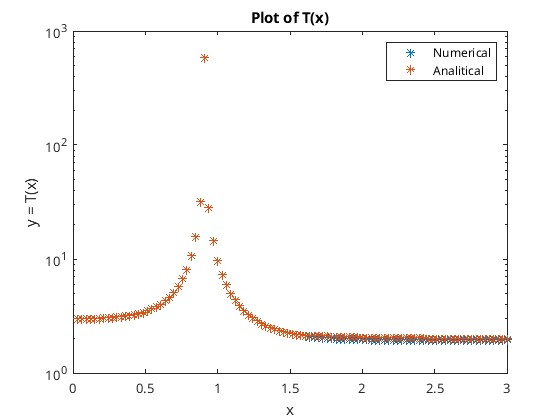
\includegraphics[width=\textwidth]{Task1.jpg}

\pagebreak
\section{Task 2}
\Lorem ipsum dolor sit amet, officia excepteur ex fugiat reprehenderit enim
labore culpa sint ad nisi Lorem pariatur mollit ex esse exercitation amet. Nisi
anim cupidatat excepteur officia. Reprehenderit nostrud nostrud ipsum Lorem est
aliquip amet voluptate voluptate dolor minim nulla est proident. Nostrud
officia pariatur ut officia. Sit irure elit esse ea nulla sunt ex occaecat
reprehenderit commodo officia dolor Lorem duis laboris cupidatat officia
voluptate. Culpa proident adipisicing id nulla nisi laboris ex in Lorem sunt
duis officia eiusmod. Aliqua reprehenderit commodo ex non excepteur duis sunt
velit enim. Voluptate laboris sint cupidatat ullamco ut ea consectetur et est
culpa et culpa duis.

\end{document}

